\documentclass[12pt, a4paper]{article}
\usepackage[utf8]{inputenc}
\usepackage{amsmath}
\usepackage{amssymb}
\usepackage{natbib}
\usepackage{mathtools}
\usepackage{titling}
\usepackage[hidelinks]{hyperref}
\usepackage{booktabs}
\usepackage{float}
\usepackage{pbox}
\usepackage{adjustbox}
\usepackage{MnSymbol}
\usepackage{wasysym}
\usepackage{geometry}

\usepackage[font={it}, labelfont=bf]{caption}
\usepackage{graphicx}

%\usepackage{setspace}
%\doublespacing

\graphicspath{ {images/} }

\author{Reid McIlroy-Young}
\title{Masters in Computational Social Science\\ \quad \\ \large Thesis Proposal}
\date{November 14, 2017}


\begin{document}
\pagenumbering{gobble}
\maketitle
\newpage
\pagenumbering{Roman}
\setcounter{page}{1}
\section{Introduction}

Currently most analysis of scientific publications is limited to those fields available in the database used by the researchers. Efforts to extend the fields usually rely on unsupervised clustering (e.g. \cite{Boyack2005}). These methods are useful and have greatly increase out understanding of how science works as a social phenomena. But, if we want to find paper with properties not given in the standard databases the usual solution is hand coding, which is either time consuming or expensive (usually both).

Recent developments in deep learning \citep{karpathy2015deep} have been highly successful at labelling/classifying very complex inputs, usually text or images. These techniques rely on large training datasets which are not available for bibliometric tasks and thus very little work has been done with scientific metadata. I have already shown that relaxing the purity requirements of the training data we shows that sufficiently large training data can be generated and that it produces useful results \citep{mcilroy2017novel}.

The classification problem I am interested in is identifying \textit{papers introducing new software packages, tools or interfaces}. This aspect of the literature has not been previously analysed like this due to data limitations. Thus this method allows me to with high confidences give broad statistics about software usage in statistics that have never been calculated before. Then move to a detailed analysis of my findings using further deep neural network, natural language processing and science studies techniques. 


\section{Literature Review}

Computer's have been a formal part of scientific work since the 18th Century \citep{grier2013computers}, but the modern day electromechanical machines developed by Turing \citep{turing1937computable} and many others \citep{abbate2012recoding}\citep{abbate2000inventing} are a much more recent innovation, of the last century \citep{bauer1972software}.  The introduction of these devices to communities around the world (both metaphorically and literally) has had major impacts on the culture \citep{lessig2007code}, technology\citep{abbate2000inventing} and rate of development \citep{bauer1972software}. Much work has been done to study these effects, but it has been primarily focused on either the macro cultural effects \citep{pfaffenberger1988social} or the economic/business usage \citep{landauer1995trouble}. 

By comparison the usage of computers by scientists has been overlooked by researchers \citep{sloanrep}. This oversight has many reasons, but one of the most significant is the lack of available data. The primary methods for large scale analysis of the culture or structure of scientific work involve bibliometric techniques \citep{de2009bibliometrics} using large standard datasets\citep[e.g.][]{Boyack2005, borner2010atlas, borner2015atlas, sugimoto2013global, shi2015weaving, evans_meta, skupin2013visualizing}. These dataset are generally lacking information about the computational aspects of the work, e.g. the  Clarivate Analytics Web of Science (WOS) does not have any such field \citep{mkdocs} and as such research into this dimension is difficult. Recent developments in natural language processing (NLP) have shown that complex concepts can be extracted reliably from text for a wide variety of tasks \citep{evans2016machine}, with some very similar to that done here \citep{foster2015tradition}.

\subsection{Information Extraction}

To extract the information about software usage from the available data requires complex NLP techniques and the best methodologies change quickly\citep{evans2016machine}. As we are primarily concerned with the classification of meta-data for a record relating it to a new software tool or not, in theory there are a large number of available techniques, as this is a simple binary classification problem \citep{james2013introduction}\citep{jurafsky2000speech}\citep{murphy2012machine}. We have considered most of the available techniques:

\begin{itemize}
\item Classified based on a simple regular grammar, e.g. regex
\item Word collocation frequencies \citep{manning1999foundations}
\item Term frequency–inverse document frequency vectors with an SVM or other classifier \citep{collobert2011natural}
\item Word2Vec vectors with an SVM or other classifier\citep{mikolov2013distributed}\citep{collobert2011natural}
\end{itemize}

The the current state of the art for natural language processing is the usage of deep neural networks for information extraction requiring more than simple word level similarities\citep{manning-EtAl}. As this is the state of the art there is no simple set of rules to follow, but there are some guidelines \citep{Goodfellow-et-al-2016}. These have lead us to the use of a recurrent neural network (RNN) \citep{mikolov2010recurrent} for the classification, although the exact specifics have been determined with cross-validation techniques \citep{james2013introduction}. The main features to consider are the type of regularization \citep{Goodfellow-et-al-2016}, what representation of words to use (most likely Word2Vec \citep{mikolov2013distributed}), what non-textual data will be included as there are in the WOS data set over 60 possible fields for each record \citep{mkdocs} and what values the hyperparameters take\citep{Goodfellow-et-al-2016}. This tuning is highly specific to the data, framework (in this case PyTorch \citep{pytorch} with NVIDIA's cuDNN \citep{chetlur2014cudnn}) and are described in further sections.

\subsection{Data Analysis}

Once the records with new software tools have been identified, we can use the existing theory of bibliometrics to look at the network structure. The literature standard approaches are to look at the structure of these nodes in the citation and authorship graphs \citep{de2002pattern}\citep{lariviere2006canadian}\citep{borgatti2009network}. This can be a computationally intensive task but tools exists that make it more practical \citep{mclevey2017introducing} so once the records have been labelled the analysis techniques are no longer novel.

The literature is silent on basic features of scientific software usage, and even when limited to only new releases there is no existing data. Thus simple measures such as per domain counts/frequencies and basic graph measurements such as the centrality will be new contributions. 

The other main question of what causes tools to be successful, has not been answered for scientists. There has been some work in the business domain \citep{xin2008software}\citep{hsu2009computer}. The adoption of new tools by businesses is theorized to follow a sigmoid pattern, with successful new entrants having three stages of usage: First they are used by early adopters and have small market penetration. Then they reach a "take off point" and the large majority of users will adopter their tools. Finally there will be slow growth in adoption again as only the laggards are left as new users \citep{xin2008software}. This is based on adopters having a Gaussian distributed chance of adopting the tool and notably this diffusion model does not require that the software have any costs for the users and allows for network effects, thus this signature is considered in our modelling.

There also has been work done examined open source projects \citep{mockus2002two} which agrees with the theory \citep{raymond1999cathedral} of open source that success is derived from openness and collaboration. This would predict that successful tools would come from highly connected groups who are working successfully with the community. This may show up as high connectedness in the co-authorship network correlating with success.

What leads to success has also be been studied in the context of ideas in the scientific literature \citep{acharya2004ideas} \citep{johntalk} or of individuals\citep{sinatra2016quantifying}. In both cases the main measure of success is the cumulative count of citations, which we can also examine on a per paper and a per author basis. We can look for the predictors of success for a new software tool by examining its citations over time and us this as our measurement for the signature. Notably \cite{sinatra2016quantifying} show a that success very unpredictable and can happen years after the paper is published. If the software records have patterns matching this model then the diffusion model may not be a good fit.

\section{Data}

The source of data used for this analysis is the  Web of Science (WOS) database hosted by Knowledge Lab. It has metadata on almost all scientific publications from 1960 to 2015, with new records being more complete. Each publication can be linked to one or more other tables each which contain other metadata than the main table, the number of entries for each table I am concerned with are shown in Table \ref{wos} and the complete database schema in Figure \ref{schema}. Access to the database is controlled by Knowledge Lab so they would need to be contacted to access it, once access rights are obtain the database is found at \href{wos2.cvirc91pe37a.us-east-1.rds.amazonaws.com}{wos2.cvirc91pe37a.us-east-1.rds.amazonaws.com} and the documentation at \href{http://docs.cloudkotta.org/dataguide/wos.html}{http://docs.cloudkotta.org/dataguide/wos.html}.

The data for WOS were collected by Thompson Reuters until 2016, when it was given to  Clarivate Analytics who now maintain it. The contemporary publications are collected from the publishers directly while older and more obscure publications are obtained from scanned copies digitalized with OCR, which is one of the factors that leads to newer publications having much higher quality data.


\begin{table} [!ht]
	\centering
	\begin{tabular}{lr}
		\toprule
		Table & Number of Entries\\
		\midrule
		publications & 57136685\\
		abstracts &	26093439\\
		publishers & 50668193\\
		keywords &	78155603\\
		references &	1085738245\\
		\bottomrule
	\end{tabular}
	\caption{Web of Science database number of entries per table}\label{wos}
\end{table}

\begin{figure}[H]
	\centering
	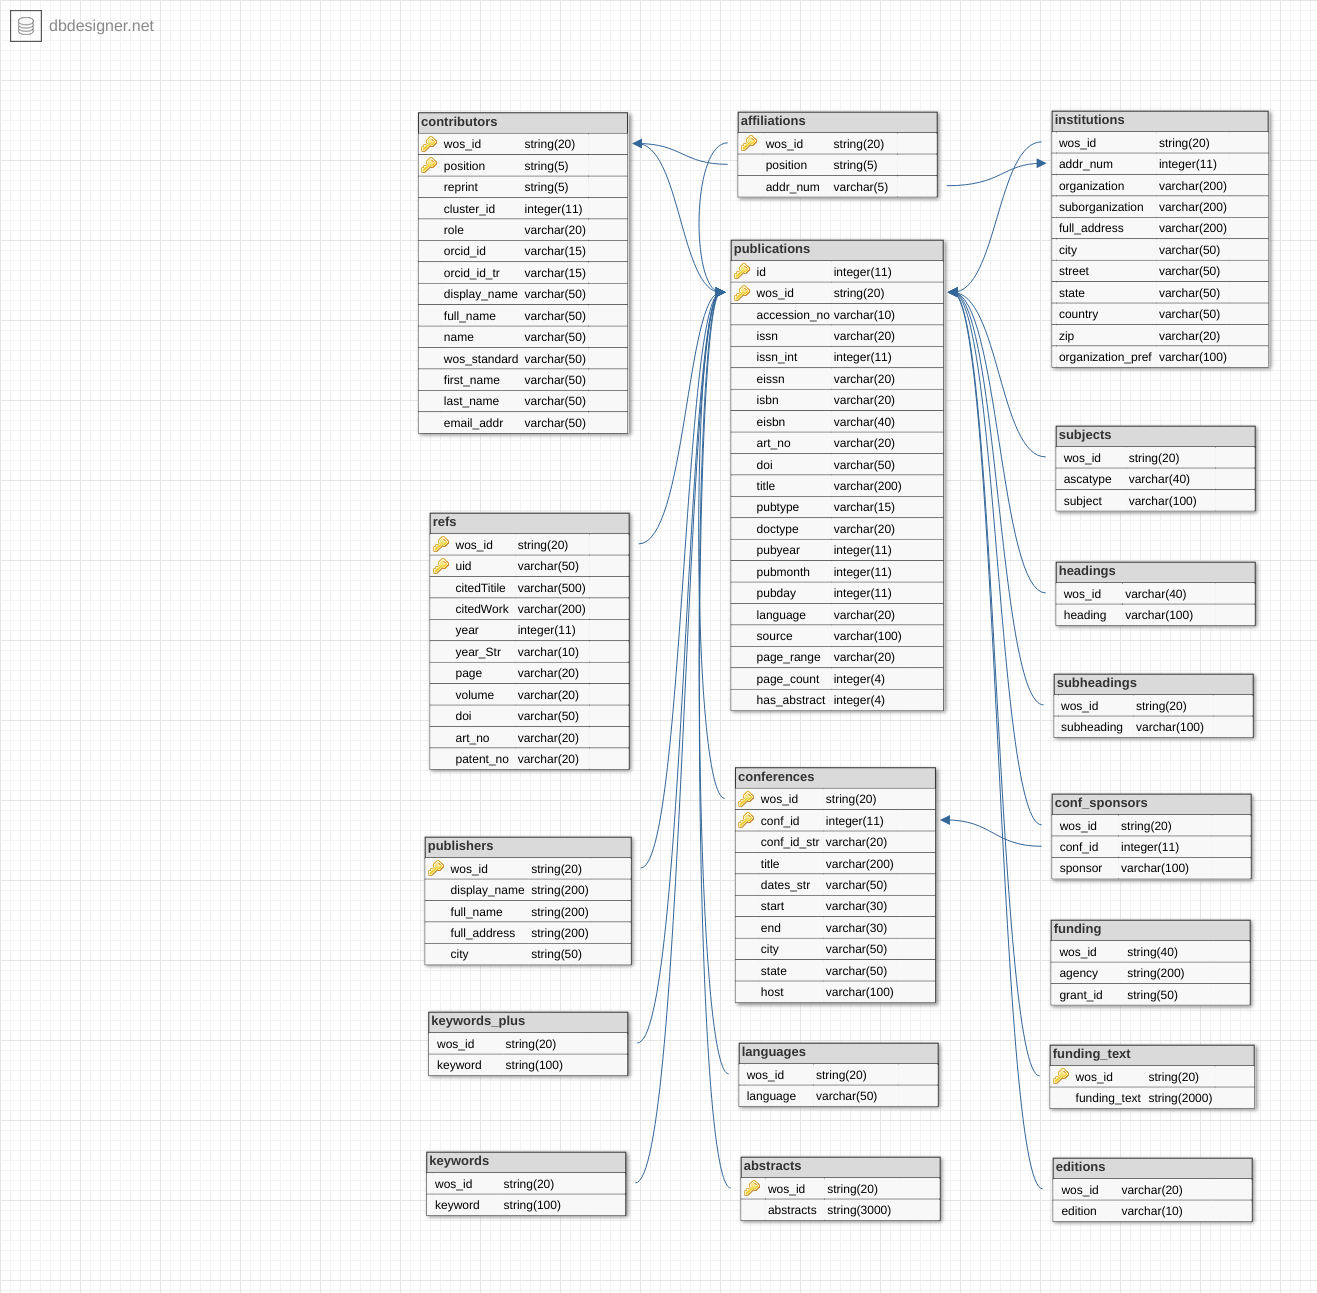
\includegraphics[width=\textwidth]{wos2_schema}
	\caption{Knowledge Lab WOS database schema}\label{schema}
\end{figure}

\section{Proposal}

For my thesis I wish to examine how scientists use and think about computational tools. To do this I will build on my own work in extracting references to new tools from scientific metadata, by both expanding the scope and depth of the study. For this work I will mostly concern myself with the title, abstract, authors, date and research area data. Already I can identify which articles in statistics journals are discussing new software tools with a good degree of accuracy. It is worth noting that, this dataset and method limits the types of computational tools I can study to those that scientists discuss in papers, which generally means programs and libraries coded by scientists who worked on the paper. Often programs and libraries are coupled to the paper, although how tight the coupling is will have to be explored. For the final paper I hope to expand to most of the social sciences and to a twenty year window (1995-2015), improve the accuracy and obtain more than a simple binary classification. With an improved model I can look at how scientists create and interact with software. If improving the model proves to be simple I also would like to look at how the plots and diagrams in the publications change over time and are generated as they are directly informed by the software tools and thus provides a window into the creator's computing environment. Another extension I hope to achieve is the addition of source code repositories (such as \href{http://github.com}{GitHub}) to my analysis, but at this point I do not know  how much access I will have to them.

Once I have my data there are many topics to explore: First how does computational tool development and uptake vary across disciplines? And are there periods of adoption or is adoption continuous? These questions are related to Galison's update \citep{galison1997image} to the Kuhnian idea of paradigm shifts \citep{kuhn1963structure}, can we observe shifts in software usage? And what components of the research is the software? Additionally, I am interested in the networks that develop around software is creation of software a normal thing for scientists to be doing or is it limited to a small (epistemic) culture \citep{cetina2009epistemic}? Finally I wish to see if the creation of software has the traditional lab structures, of the relevant field or if it is a divergent practice.

\newpage
\bibliography{Report}{}
%\bibliographystyle{plain}
\bibliographystyle{asr}

\end{document}